%%%%%%%%%%%%%%%%%%%%%%%%%%%%%%%%%%%%%%%%%
% University/School Laboratory Report
% LaTeX Template
% Version 3.1 (25/3/14)
%
% This template has been downloaded from:
% http://www.LaTeXTemplates.com
%
% Original author:
% Linux and Unix Users Group at Virginia Tech Wiki 
% (https://vtluug.org/wiki/Example_LaTeX_chem_lab_report)
%
% License:
% CC BY-NC-SA 3.0 (http://creativecommons.org/licenses/by-nc-sa/3.0/)
%
%%%%%%%%%%%%%%%%%%%%%%%%%%%%%%%%%%%%%%%%%

%----------------------------------------------------------------------------------------
%	PACKAGES AND DOCUMENT CONFIGURATIONS
%----------------------------------------------------------------------------------------

\documentclass{article}

\usepackage[version=3]{mhchem} % Package for chemical equation typesetting
\usepackage{siunitx} % Provides the \SI{}{} and \si{} command for typesetting SI units
\usepackage{graphicx} % Required for the inclusion of images
\usepackage{natbib} % Required to change bibliography style to APA
\usepackage{amsmath} % Required for some math elements 
\usepackage[utf8]{inputenc} % slovenski znaki
\usepackage[slovene]{babel} % slovenski formati
\usepackage[]{algorithm2e}
\usepackage{hyperref}
\setlength\parindent{0pt} % Removes all indentation from paragraphs

\renewcommand{\labelenumi}{\alph{enumi}.} % Make numbering in the enumerate environment by letter rather than number (e.g. section 6)

%\usepackage{times} % Uncomment to use the Times New Roman font

%----------------------------------------------------------------------------------------
%	DOCUMENT INFORMATION
%----------------------------------------------------------------------------------------

\title{Klasifikacija ploskev} % Title

\author{Rok Koleša, Domen Kren, Darko Janković} % Author name

\date{\today} % Date for the report

\begin{document}

\maketitle % Insert the title, author and date

\begin{center}
\begin{tabular}{l r}
Mentor: & as. dr. Gregor Jerše % Instructor/supervisor
\end{tabular}
\end{center}

% If you wish to include an abstract, uncomment the lines below
% \begin{abstract}
% Abstract text
% \end{abstract}

\newpage
\tableofcontents
\newpage
%----------------------------------------------------------------------------------------
%	SECTION 1
%----------------------------------------------------------------------------------------

\section{Cilj}
Cilj projekta je bil ustvariti program za klasifikacijo ploskev z robovi.

\subsection{Definicije}
\label{definicije}
\begin{description}
\item[Ploskev]
Ploskev v matematiki pomeni dvorazsežno tvorbo v večrazsežnem prostoru. Tvorba mora biti kompaktna in povezana.
\item[Robna komponenta]
Komponenta, ki predstavlja luknjo v triangulaciji. Sestavljajo jo robovi, ki so rob natanko enega trikotnika.
\end{description} 
 
%----------------------------------------------------------------------------------------
%	SECTION 2
%----------------------------------------------------------------------------------------

\section{Vhodni podatki}
Abstraktni simplicialni kompleksi, podani kot seznami trojic števil. Vsak element je celo število, ki predstavlja indeks oglišča, celotna trojica pa predstavlja trikotnik v kompleksu.
\\\\
Primer vhoda za disk:  \\
-----------------  \\
1 2 3 \\
2 3 4 \\
2 4 5 \\
2 5 6 \\
-----------------  \\
%----------------------------------------------------------------------------------------
%	SECTION 3
%----------------------------------------------------------------------------------------

\section{Rešitev}
Program za klasifikacijo ploskev je sestavljen iz treh delov: prvi preveri, če vhodna triangulacija predstavlja ploskev, drugi del prešteje robne komponente, tretji pa jo klasificira.
\subsection{Ali je triangulacija ploskev}
Najprej bomo preverili ali podana triangulacija predstavlja ploskev. V našem primeru se to prevede na preverjanje ali triangulacija predstavlja več komponent in koliko sosedov ima vsak rob. Oba algoritma sta precej preprosta. 

Pri prvem vzamemo nek trikotnik in mu dodamo sosede, nato dodamo njihove sosede, itd. Na koncu le pogledamo ali so v množici podanih trikotnikov ostali kakšni, ki jih s tem pregledovanjem nismo dosegli. Če obstajajo, imamo več komponent, česar ne moremo klasificirati.

Pri drugem pa se sprehodimo po vseh robovih trikotnikov in pogledamo ali imajo za soseda natanko enega (je del robne komponente), ali dva (rob je v ploskvi) trikotnika. Če najdemo več sosedov, triangulacija ne predstavlja ploskve.

\subsection{Število robnih komponent}
Število robnih komponent oz. število lukenj smo poiskali s preprostim algoritmom, ki je v grobem sestavljen iz naslednjih korakov:
\begin{enumerate}
\item poišči robove, ki se v triangulaciji pojavijo le enkrat
\item preštej cikle, ki jih sestavljajo dobljeni robovi
\end{enumerate}
Opisan algoritem bi na triangulaciji, prikazani na sliki \ref{triangulacija}, v primeru odstranjenih trikotnikov \textit{(2, 6, 5)} in \textit{(6, 7, 9)} našel naslednje robove, ki se pojavijo samo enkrat: \textit{2 - 5}, \textit{2 - 6} in \textit{5 - 6}, ter \textit{6 - 7}, \textit{6 - 9} in \textit{6 - 9}, iz česar bi potem zaznal dva cikla, ki sta identična odstranjenima trikotnikoma.
\begin{figure}[htb]
\begin{center}
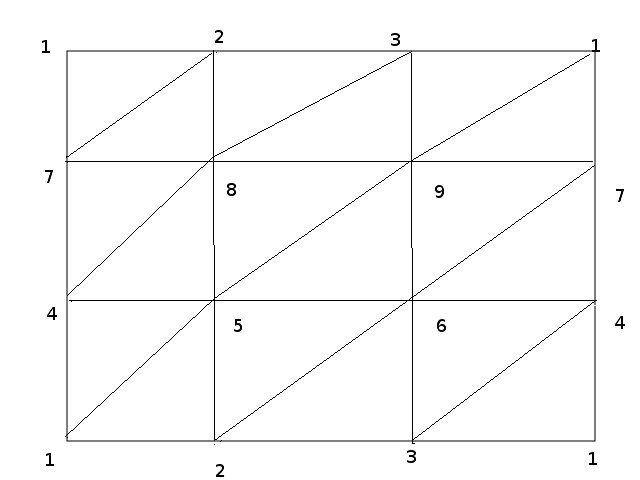
\includegraphics[scale=0.35]{Triangulation.png}
\caption{Primer triangulacije}
\label{triangulacija}
\end{center}
\end{figure}

\subsection{Klasifikacija}
Na koncu je prišla na vrsto še dejanska klasifikacija ploskve. Na vajah smo že pokazali kako se klasificira ploskve brez roba, in sicer lahko to naredimo na podlagi Eulerjeve karakteristike $\chi(T)$, kjer je $T$ triangulacija, in orientabilnosti triangulacije. Videli smo že, da se vse ploskve razdelijo na 3 različne razrede:
\begin{enumerate}
\item sfera - je orientabilna, $\chi(T)=2$ 
\item $n$ torusov - je orientabilna, $\chi(T)=2-2n$
\item $n$ projektivnih ravnin - ni orientabilna, $\chi(T)=2-n$
\end{enumerate}
Tu pa imamo opravka s ploskvami, ki mogoče vsebujejo kakšno robno komponento. Ideja za klasifikacijo takšnih ploskev pa je, da zapolnimo vse robne komponente in dobimo novo ploskev $T'$, ki pa ne vsebuje robov. Če vzamemo še orientacijo originalne triangulacije $T$ in Eulerjevo karakteristiko nove, $\chi(T')$, lahko torej dokončno klasificiramo ploskev, ki jo določa $T$.

Ostane nam torej samo še premislek za koliko se spremeni Eulerjeva karakteristika, ko tako polnimo luknje v triangulaciji. Luknjo lahko zapolnimo na 2 preprosta načina. Prvi način je ta, da na sredini neke luknje naredimo novo oglišče in iz te točke napeljemo rob na vsako oglišče na robu luknje. Drug način pa je, da iz poljubne točke napeljemo rob do vsake še ne sosednje točke. Oba načina sta pokazana na sliki \ref{luknje} na primeru, ko ima rob 10 oglišč.

\begin{figure}[htb]
\begin{center}
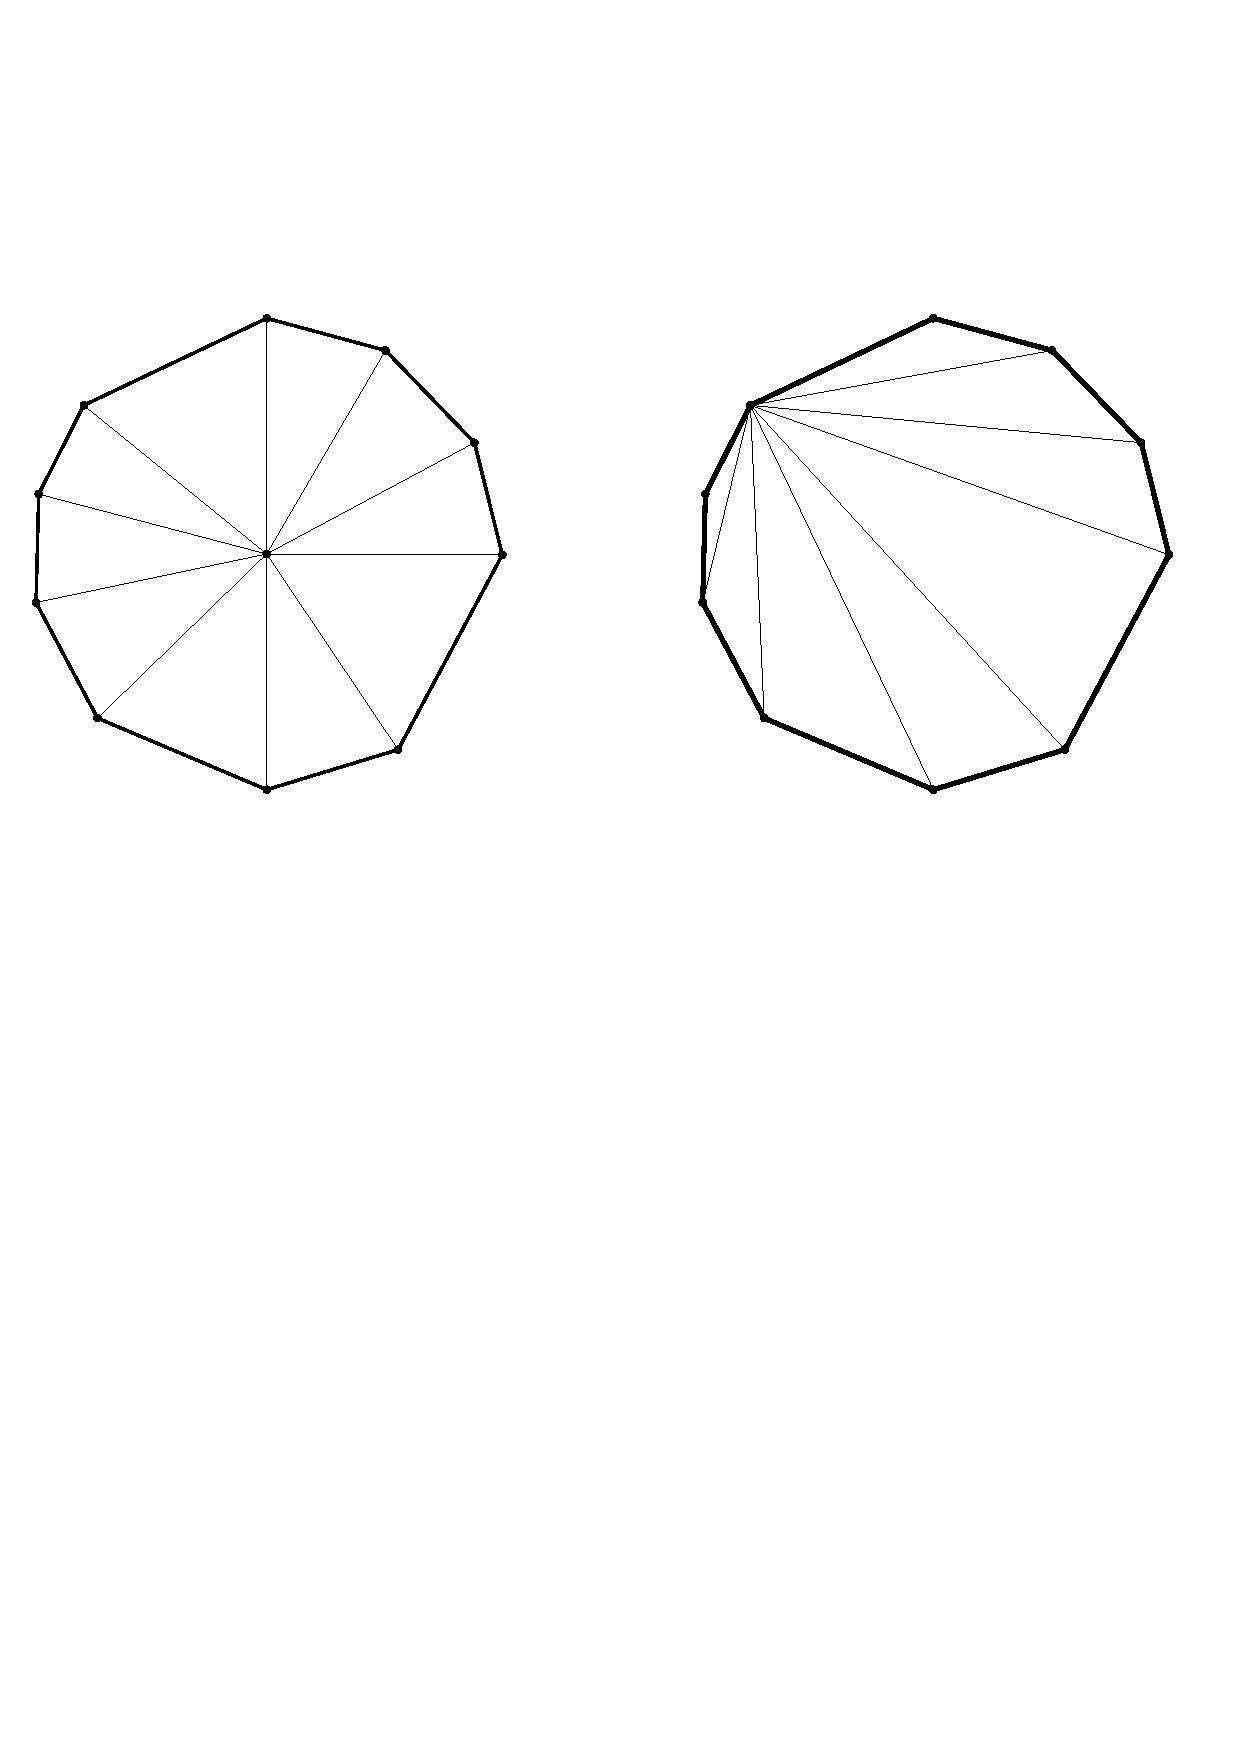
\includegraphics[scale=0.5]{luknje.pdf}
\caption{Dva načina polnjena luknje}
\label{luknje}
\end{center}
\end{figure}

Poglejmo sedaj koliko smo "pokvarili" Eulerjevo karakteristiko. Recimo, da ima robna komponenta $m$ oglišč. Pri prvem načinu smo dodali 1 oglišče in za vsako oglišče robne komponente en rob, torej $m$ robov. S tem smo za vsak rob robne komponente (ki jih je enako kot oglišč, torej $m$) tudi dodali en trikotnik. Obstoječih simpleksov nismo kvarili in zato se Eulerjeva karakteristika glasi:
$$\chi(T')=\chi(T) + 1 - m + m = \chi(T) + 1$$
Pri drugem načinu pa dodamo vse diagonale iz neke točke kot robove. Teh je tako $m-3$, saj ne moremo napeljati diagonale z direktnimi sosedi (ta rob v $T$ namreč že obstaja) in tudi ne sam s sabo. Ker ima robna komponenta tudi $m$ robov, bomo dobili $m-2$ novih trikotnikov, saj samo z dvema robovoma (sosednima) ne moremo dobiti trikotnika. Novh točk nismo dodali in zato je Eulerjeva karakteristika enaka
$$\chi(T')=\chi(T) + 0 - (m-3) + m-2 = \chi(T) + 3 - 2 = \chi(T) + 1.$$
V obeh primerih smo pričakovano dobili enak rezultat, torej se $\chi(T)$ pri polnjenju ene luknje spremeni za 1.

Zaključimo torej, da je dovolj če izračunamo $\chi(T)$ in tej številki dodamo število robnih komponent, da dobimo $\chi(T')$. Sedaj lahko popolnoma klasificiramo vse ploskve z robom in brez.

%----------------------------------------------------------------------------------------
%	SECTION 4
%----------------------------------------------------------------------------------------

\section{Rezultati}
Algoritem smo pognali na podanih testnih primerih. Rezultati testov so naslednji:
\begin{enumerate}
\item Klasifikacija triangulacije iz datoteke SyrfaceK.txt \\
	Podana ploskev je 2 projektivnih ravnin s/z 0 luknjami
\item Klasifikacija triangulacije iz datoteke space\_stationSurface.txt \\
	Podana sta dva identična trikotnika: Trikotnik: (6366, 6367, 6368) in Trikotnik: (6368, 6367, 6366). Podan vhod ni ploskev.
\item Klasifikacija triangulacije iz datoteke space\_stationSurface\_no\_duplicates.txt \\
	Triangulacija ima več komponent! \\
	Podana triangulacija ne predstavlja ploskve
\item Klasifikacija triangulacije iz datoteke disc.txt \\
	Podana ploskev je sfera s/z 1 luknjami
\item Klasifikacija triangulacije iz datoteke SurfaceT.txt \\
	Podana ploskev je 1 torusov s/z 0 luknjami
\item Klasifikacija triangulacije iz datoteke SurfaceGJ1.txt \\
	Podana ploskev je 1 torusov s/z 0 luknjami
\item Klasifikacija triangulacije iz datoteke SurfaceGJ2.txt \\
	Podana ploskev je 2 projektivnih ravnin s/z 0 luknjami
\end{enumerate}

%----------------------------------------------------------------------------------------
%	SECTION 5
%----------------------------------------------------------------------------------------

\section{Zaključek}
S projektnim delom smo dosegli klasifikacijo ploskve z morebitnim robom. Seveda mora podan abstraktni simplicialni kompleks sploh predstavljati ploskev. Nato je treba poiskati le orientacijo ploskve in robne komponente. Za oboje se lahko uporabi preprosta algoritem (za orientacijo smo že spoznali na vajah), ostalo pa tudi ni težko implementirati. Luknje se da zapolniti tudi na drugačne načine, opisana pa sta dva najbolj intuitivna.

Implementacija tega projekta je potekala v Javi verzije 8. Vsa koda vključno s testnimi primeri pa so dostopni tudi na GitHub-u:\\ \url{https://github.com/dokren/SurfaceClassification/}


\end{document}